\textit{Netcat}, normalmente abreviado a \textit{nc}\cite{netcat} es una utilidad de red para leer y escribir en conexiones de red utilizando \acrshort{tcp} o \acrshort{udp}. El comando está diseñado para ser un backend confiable que puede ser usado directamente o fácilmente manejado por otros programas y scripts. Al mismo tiempo, es una herramienta de investigación y depuración de redes con muchas características, ya que puede producir casi cualquier tipo de conexión que su usuario pueda necesitar y tiene una serie de capacidades incorporadas.\\

Algunas de las principales características de \textit{netcat} son
\begin{itemize}
    \item Conexiones salientes o entrantes, \acrshort{dns} o \acrshort{udp}, hacia o desde cualquier puerto.
    \item Comprobación completa de \acrshort{dns}.
    \item Posibilidad de utilizar cualquier puerto de origen local.
    \item Posibilidad de utilizar cualquier dirección de origen de red configurada localmente.
    \item Capacidad incorporada de enrutamiento de origen.
    \item Puede leer los argumentos de la línea de comandos desde la entrada estándar.
    \item Volcado hexadecimal de los datos transmitidos y recibidos.
    \item Capacidad opcional de dejar que otro programa atienda las conexiones establecidas.
\end{itemize}

Como se muestra en la figura \ref{fig:ayuda-nc}, \textit{Netcat} tiene las siguientes opciones de uso:
\begin{figure}[h]
    \centering
    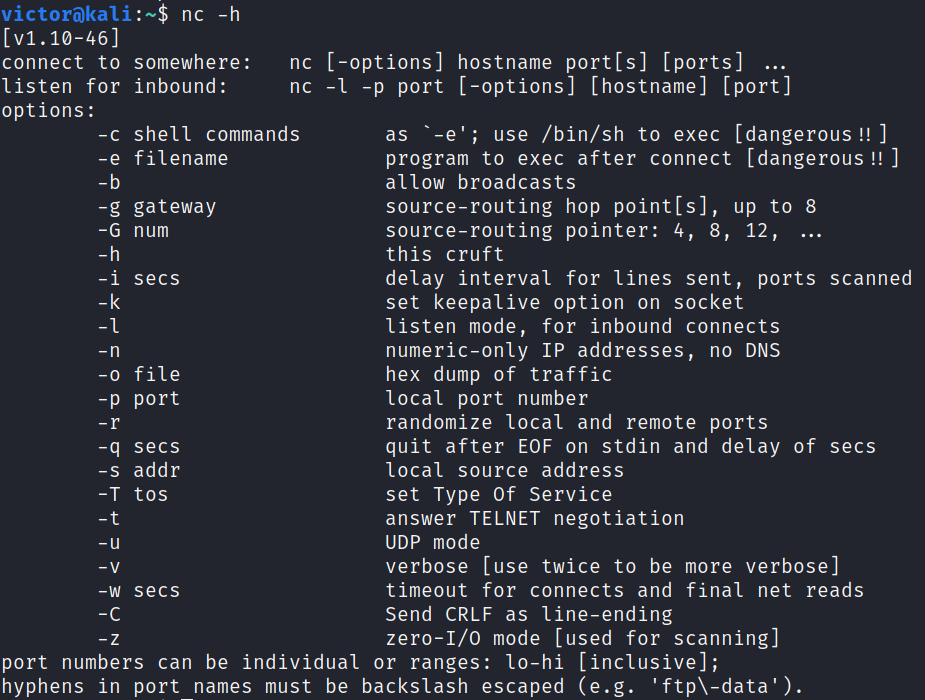
\includegraphics[width=0.8\textwidth]{images/sections/tools/nc-help.png}
    \caption{Ayuda de \textit{Netcat}}
    \label{fig:ayuda-nc}
\end{figure}